\section{Lebesgue measure}

Consider a closed interval in $\mathbb{R}$,
\begin{align}\label{closed_interval}
    P = [a_1,b_1] \times \cdots [a_n,b_n] \subset \mathbb{R}^n,
\end{align}
and we define its volume as 
\begin{align*}
    \left|P\right| \coloneqq (b_1-a_1) \cdots (b_n-a_n).
\end{align*}

\medskip

\begin{definition}
For any $A \subset \mathbb{R}^n$, the outer Lebesgue measure of $A$ is defined as
\begin{align*}
    \mathcal{L}^*_n(A) = \inf \sum^\infty_{i=1} \left|P_i\right|,
\end{align*}
where the infimum is taken over all coverings 
\begin{align*}
    A \subset \bigcup^\infty_{i=1} P_i,
\end{align*}
by intervals as in (\ref{closed_interval}). $\mathcal{L}^*_n$-measurable sets are called Lebesgue measurable. $\mathcal{L}^*_n$ restricted to Lebesgue measurable sets is called Lebesgue measure and is denoted by $\mathcal{L}_n$.
\end{definition}

\medskip

\begin{theorem}
$\mathcal{L}^*_n$ is a metric outer measure.
\end{theorem}

\medskip

\begin{remark}
By Theorem \ref{theorem_113}, $\BB(\mathbb{R}^n)$ is Lebesgue measurable.
\end{remark}

\medskip

\begin{corollary}
All Borel sets in $\mathbb{R}^n$ are Lebesgue measurable. 
\end{corollary}

\medskip

Recall that if $\mu^*$ is an outer measure, by Proposition \ref{prop_14}, all sets $A$ such that $\mu^*(A) = 0$ are $\mu^*$-measurable. Therefore, if $\mathcal{L}^*_n(A) = 0$, then $A$ is Lebesgue measurable, and $\mathcal{L}_n(A) = 0$. Note that $\mathcal{L}_n(A) = 0$ if and only if for all $\varepsilon > 0$, there is a family of closed intervals $\{P_i\}$ such that 
\begin{align*}
    A \subset \bigcup^\infty_{i=1} P_i, \quad \text{and} \quad \sum^\infty_{i=1} \left|P_i\right| < \varepsilon.
\end{align*}

\medskip

\begin{theorem}\label{theorem_125}
If $P$ is a closed interval as in (\ref{closed_interval}), then $\mathcal{L}_n(P) = \left|P\right|$.
\end{theorem}

We often write $\left|A\right|$ to denote the Lebesgue measure of a Lebesgue measurable set $A$.

\begin{proof}
By definition,
\begin{align*}
    \mathcal{L}_n(P) = \inf \sum^\infty_{i=1} \left|P_i\right|, \quad P \subset \bigcup^\infty_{i=1} P_i.
\end{align*}
Taking covering of $P$ by itself, then $P \subset P$, then $\mathcal{L}_n(P) \leq \left|P\right|$.

It remains to show that $\left|P\right| \leq \sum^\infty_{i=1} \left|P_i\right|$. And we need a lemma to prove this.

\begin{lemma}\label{lemma_121}
If $P \subset \bigcup^k_{i=1} P_i$ is a finite covering of a closed interval $P$ by closed intervals $P_i$, then $\left|P\right| \leq \sum^k_{i=1} \left|P_i\right|$.
\end{lemma}
\begin{proof}[``Proof'']
We use the Riemann integral to prove this. Since $P \subset \bigcup^k_{i=1} P_i$, then
\begin{align*}
    \chi_P \leq \sum^k_{i=1} \chi_{P_i}.
\end{align*}
Then, we have
\begin{align*}
    \left|P\right| = \int_{\mathbb{R}^n} \chi_P \leq \sum^k_{i=1} \int_{\mathbb{R}^n} \chi_{P_i} = \sum^k_{i=1} \left|P_i\right|.
\end{align*}
\end{proof}
\begin{figure}[H]
    \centering
    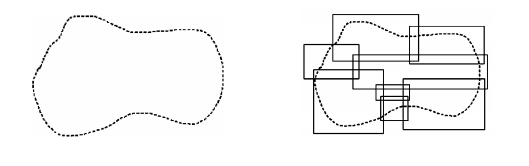
\includegraphics[width=0.6\textwidth]{closed_interval_covering.png}
    \caption{Example of a set covered by intervals.(From \cite{6})}
    \label{fig:closed_intervals}
\end{figure}

Now we can complete the proof of the theorem. Each interval $P_i$ is contained in a slightly bigger open interval $P_i^\varepsilon$ such that
\begin{align*}
    \left|\overline{P_i^\varepsilon}\right| = \left|P_i\right| + \frac{\varepsilon}{2^i},
\end{align*}
where $\overline{P_i^\varepsilon}$ is the closure of $P_i^\varepsilon$. Since $P$ is compact, then we can select a finite subcovering 
\begin{align*}
    P \subset \bigcup^k_{j=1} P_{i_j}^\varepsilon,
\end{align*}
and the lemma implies
\begin{align*}
    \left|P\right| \leq \sum^k_{j=1} \left|\overline{P_{i_j}^\varepsilon} \right| \leq \sum^\infty_{j=1} \left| \overline{P_{i}^\varepsilon} \right| = \sum^\infty_{i=1} \left|P_{i}\right| + \varepsilon,
\end{align*}
since $\varepsilon > 0$ is arbitraty, then the theorem follows.
\end{proof}

\medskip

\begin{proposition}
Let $P$ ba an open interval.
\begin{enumerate}
    \item[(a)] If $P = (a_1,b_1) \times \cdots (a_n,b_n)$ is a bounded interval, then 
    \begin{align*}
        \mathcal{L}_n(P) = (b_1-a_1) \cdots (b_n-a_n).
    \end{align*}
    
    \item[(b)] $\mathcal{L}_n(\partial P) = 0$.
    
    \item[(c)] If $P$ is an unbounded interval in $\mathbb{R}_n$ and has nonempty interior (i.e. each side has positive length and at least one of the sides has infinite length, which is of form $(-\infty,b), (a,\infty)$ or $(-\infty,\infty)$), then $\mathcal{L}_n(P) = \infty$.
\end{enumerate}
\end{proposition}
\begin{proof}
~\begin{enumerate}
    \item[(a)] For $P$, we could find a slightly smaller interval $P_\varepsilon$ contained in $P$ and a slightly bigger interval $P^\varepsilon$ which contains $P$, where\footnote{Here, $\bigtimes$ denotes the Cartesian product.}
    \begin{align*}
        P_\varepsilon = \bigtimes^n_{i=1} \left[a_i+\varepsilon,b_i-\varepsilon\right], \quad P^\varepsilon = \bigtimes^n_{i=1} \left[a_i-\varepsilon,b_i+\varepsilon\right].
    \end{align*}
    Then, $\mathcal{L}_n(P_\varepsilon) \leq \mathcal{L}_n(P) \leq \mathcal{L}_n(P^\varepsilon)$. Letting $\varepsilon \to 0$ yields the result:
    \begin{align*}
        (b_1-a_1) \cdots (b_n-a_n) \leftarrow \mathcal{L}_n(P_\varepsilon) \leq \mathcal{L}_n(P) \leq \mathcal{L}_n(P^\varepsilon) \to (b_1-a_1) \cdots (b_n-a_n).
    \end{align*}
    
    \item[(b)] $\mathcal{L}^n(\partial P) =  \mathcal{L}^n(\overline{P}) - \mathcal{L}^n(\operatorname{int}(P)) = 0$.
    
    \item[(c)] $P$ contains closed intervals of arbitrarily large measure.
\end{enumerate}
\end{proof}

\medskip

\begin{corollary}\label{coro_1261}
If $k < n$, then $\mathcal{L}_n (\mathbb{R}^k) = 0$.
\end{corollary}
\begin{proof}
It suffice to show that $[-k,k]^{k} \times \{0\}^{n-k}$ has Lebesgue measure zero for all $k \in \mathbb{N}$.\footnote{It is based on the proof of  $\mathbb{R}^n\times\{0\}$ has measure zero in $\mathbb{R}^{n+1}$: \url{https://math.stackexchange.com/a/524155}.} 

For any $\varepsilon > 0$, choose $\delta > 0$ such that
\begin{align*}
    (2\delta)^{n-k} (2k+2\varepsilon)^k < \varepsilon.
\end{align*}
Now we define $$U_k = (-k-\varepsilon,k+\varepsilon)^k \times (-\delta,\delta)^{n-k},$$ 
and clearly $U_k$ contains $[-k,k]^{k} \times \{0\}^{n-k}$. Also, by the choice of $\delta$, $\mathcal{L}_n(U_k) < \varepsilon$, and since
\begin{align*}
    \mathcal{L}_n(\mathbb{R}^k) = \lim_{k\to\infty} \mathcal{L}_n\left([-k,k]^{k} \times \{0\}^{n-k}\right) < \varepsilon,
\end{align*}
we have $\mathcal{L}_n(\mathbb{R}^k) = 0$.
\end{proof}

\medskip

\begin{proof}[Second Proof of Corollary \ref{coro_1261}]
Finite intervals in $\mathbb{R}^k$ are contained in $\partial P$ for some interval $P$ in $\mathbb{R}^n$. Then, finite intervals in $\mathbb{R}^k$ have Lebesgue measure zero. Since $\mathbb{R}^k$ is a union of finite intervals in $\mathbb{R}^k$, then $\mathcal{L}^n(\mathbb{R}_k) = 0$.
\end{proof}

\medskip

\begin{theorem}
For an arbitrary set $E \subset \mathbb{R}^n$ (not necessarily measurable),
\begin{align*}
    \mathcal{L}_n^*(E) = \inf_{\substack{U \subset E\\ U - \text{open}}} \mathcal{L}_n(U).
\end{align*}
\end{theorem}
\begin{proof}
Clearly, $\mathcal{L}_n^*(E) \leq \inf_{U \subset E} \mathcal{L}_n(U)$. It remains to show the other direction.

By definition, $\mathcal{L}^*_n(E) = \inf \sum^\infty_{i=1} \left|P_i\right|$, $E \subset \bigcup_i P_i$, where $P_i$ are closed intervals. Now let $P_i^\varepsilon$ be open interval such that $P_i \subset P_i^\varepsilon$ and
\begin{align*}
    \left|P_i^\varepsilon\right| = \left|P_i\right| + \frac{\varepsilon}{2^i}.
\end{align*}

This approximation yields
\begin{align*}
    \mathcal{L}_n^*(E) = \inf \sum^\infty_{i=1} \left|P_i\right|, \quad E \subset \bigcup^\infty_{i=1} P_i,
\end{align*}
where $P_i$ are open. Indeed, by the subadditivity of the outer measure, $\mathcal{L}_n^*(E) \leq \sum^\infty_{i=1} \left|P_i\right|$, which implies $\mathcal{L}_n^*(E) \leq \inf \sum^\infty_{i=1} \left|P_i\right|$. Also, every closed interval can be approximated by a slighter bigger open interval, and this implies the equality.

Now, for $E \subset \bigcup^\infty_{i=1}P_i$, $P_i$ are open intervals, by Theorem \ref{theorem_125},
\begin{align*}
    \sum^\infty_{i=1} \left|P_i\right| \geq \left|\bigcup^\infty_{i=1}P_i\right| = \mathcal{L}_n\left(\bigcup^\infty_{i=1}P_i\right) \geq \inf_{U \supset E} \mathcal{L}_n(U),
\end{align*}
where $U$ is open, and taking the infimum over all coverings $E \subset \bigcup^\infty_{i=1}P_i$ by open intervals yields
\begin{align*}
    \mathcal{L}_n^*(E) \geq  \inf_{U \supset E} \mathcal{L}_n(U).
\end{align*}
\end{proof}

\medskip

So how to compute $\mathcal{L}_n(U)$ for open set $U$? Let's introduce the dyadic cubes. Consider cubes vertices in $\mathbb{Z}^n$, and divide each cubes into $2^k$ cubes, $k = 0,1,2,\cdots$. 

\medskip

\begin{theorem}
An arbitrary open set in $\mathbb{R}^n$ is a union of closed dyadic cubes with pairwise disjoint interiors. Then the Lebesgue measure of the open set equals the sum of the measures of these cubes.
\end{theorem}
\begin{figure}[H]
    \centering
    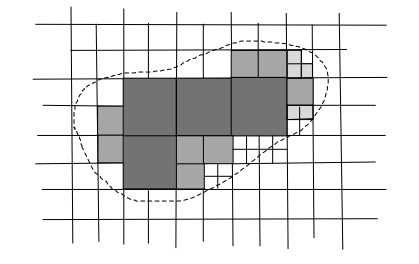
\includegraphics[width=0.5\textwidth]{dyadic_cube.png}
    \caption{Example of open set represented by the dyadic cubes in $\mathbb{R}^2$.(From \cite{6})}
    \label{fig:dyadic_cube}
\end{figure}

\medskip

Recall that by a $G_\delta$ set we mean a set of the form $G = \bigcap^\infty_{i=1} G_i$, where $G_i \subset X$ are open and by a $F_\sigma$ set we mean a set of the form $F = \bigcap^\infty_{i=1} F_i$, where $F_i \subset X$ are closed. Clearly, all $G_\delta$ and $F_\sigma$ sets are Borel sets.

\medskip

\begin{theorem}
Let $A \subset \mathbb{R}^n$, then the following conditions are equivalent:
\begin{enumerate}[label=(\alph*)]
    \item $A$ is Lebesgue measurable;
    
    \item For every $\varepsilon > 0$, there is an open set $G$ such that $A \subset G$ and $\L^*_n(G\setminus A) = 0$;
    
    \item There is a $G_\delta$ set $H$ such that $A \subset H$ and $\L^*_n(H\setminus A) < \varepsilon$;
    
    \item For every $\varepsilon > 0$, there is a closed set $F$ such that $F \subset A$ and $\L^*_n(A\setminus F) < \varepsilon$;
    
    \item There is a $F_\sigma$ set $M$ such that $M \subset A$ and $\L^*_n(A\setminus M) = 0$;
    
    \item For every $\varepsilon > 0$, there is an open set $G$ and a closed set $F$ such that $F \subset A \subset G$ and $\L_n(G \setminus F) < \varepsilon$.
\end{enumerate}
\end{theorem}
\begin{proof}
~\begin{enumerate}
    \item[(a)]$\Rightarrow$ (b) Every measurable set can be represented as a union of sets with finite measure $A = \bigcup^\infty_{i=1}A_i$, $\L_n(A_i) < \infty$, where $A_i$ is Lebesgue measurable and $\L_n(A_i) < \infty$. Indeed, since $A$ is arbitrary Lebesgue measurable set, then we can define $A_i = A \cap B(0,i), i = 1,2,\cdots,n$, where $B(0,i) \subset \mathbb{R}^n$ is the closed ball centered at the origin with radius $i$.
\end{enumerate}
\end{proof}